
%----------------------------------------------------------------------------------------
%	Lecture 22
%----------------------------------------------------------------------------------------

\chapter{Triple Integrals in Spherical Coordinates} 

\bigbreak

\section{Spherical Coordinates}

Spherical Coordinates are $(r, \phi, \theta)$ where $r$ is the distance from the origin, 
$\phi$ is the angle between the position vector and the positive $z$-axis 
and $\theta$ is the angle between the projection of the position vector onto the $XY$-plane and the position $x$-axis.


\begin{figure}[ht!]
    \centering
    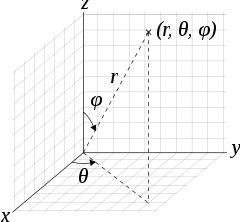
\includegraphics[scale=0.7]{./images/lecture_22_figure_1.png}
    \caption{Spherical Coordinates}
\end{figure}


Here, $r = a$ is the equation of a sphere of radius $a$ then $\theta$ denotes the latitute and $\phi$ denotes the longitude.


The above images gives us the key to convert between spherical coordinates and cyclidrical coordinates.
We can see that the vertical distance of the point from the $XY$-plane will be $r \cos \phi$.
And the distance between the projection of the point on the $XY$-plane and the origin will be $r \sin \phi$.

Thus we get our cyclidrical coordinates as $(r, \theta, z) = (r \sin \phi, \theta, r \cos \phi)$. 
We can continue to convert these into cartesian coordinates as well.


Here, $\theta = \theta_0$ is the equation of a half plane starting at the $z$-axis.
And $\phi = \phi_0$ is the equation of a cone pointing up for $\phi_0 < \pi / 2$ and pointing down for $\phi_0 > \pi / 2$.
For $\phi = \pi/2$ is the $XY$-plane.

Finally, in cartesian coordinates $x = r \sin \phi \cos \theta$, $y = r \sin \phi \cos \theta$ and $z = r \cos \phi$.

\pagebreak

\section{Triple Integral in Spherical Coordinates}

Our volume element will be $\Delta V \propto \Delta r \Delta \phi \Delta \phi$. 
Let's start by fixing $r$ and try to find out the surface area element corresponding to $\Delta \theta$ and $\Delta \phi$.

\begin{figure}[ht!]
    \centering
    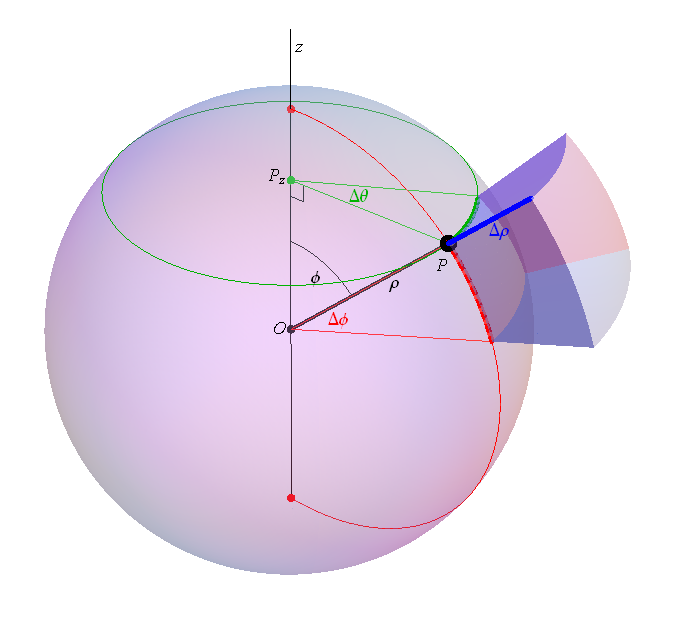
\includegraphics[scale=0.3]{./images/lecture_22_figure_2.png}
    \caption{Volume Element In Spherical Coordinates ($\rho$ is the same as $r$)}
\end{figure}

Here the surface area element will be equal to the product of the length of the red and green segment.

We can see that the red segment is a piece of the red circle whose raduis is $r$ so the red segment will be $r \Delta \phi$.
Also the green segment is the piece of the green circle whose raduis is $r \sin \phi$ so the green segment is $r \sin \phi \Delta \theta$.

Thus, the area element is $\Delta A = r^2 \sin \phi \Delta \theta \Delta \phi$.

Finally for the volume element we can multiply the area element by $\Delta r$ to get $\Delta V = r^2 \sin \phi \Delta r \Delta \phi \Delta \theta \Rightarrow dV = r^2 \sin \phi dr d\phi d\theta$.


